\documentclass[12pt,a4paper]{report}

% ===========================================================================
% THESIS OUTLINE / SKELETON
% 3D House Defense Game — a vehicle for Business Analysis & Frontend skills
% ---------------------------------------------------------------------------
% HOW TO USE THIS FILE
%   * This is a STRUCTURE you drop into your existing thesis template.
%   * Top-level entries are \chapter (matching your template's numbered
%     "1 INTRODUCTION", "2 OBJECTIVES", ... ). If your template uses \section
%     for those instead, demote every level by one (\chapter->\section, etc.).
%   * Under each heading is a short paragraph describing what to write there
%     (the "few lines of introduction" you asked for) — keep it, expand it,
%     or replace it.
%   * Blue notes marked  >  flag where a TABLE, FIGURE or DIAGRAM belongs.
%     Search this file for "\needfig" and "\needtab" to find them all.
% ===========================================================================

\usepackage[utf8]{inputenc}
\usepackage[T1]{fontenc}
\usepackage[margin=1in]{geometry}
\usepackage{amsmath}
\usepackage{graphicx}   % for \resizebox and the cover logo
\usepackage{xcolor}
\usepackage{float}      % for the [H] figure placement
\usepackage{tikz}
\usetikzlibrary{arrows.meta, shapes.geometric, positioning, calc}
\usepackage{hyperref}
\hypersetup{colorlinks=true, linkcolor=black, urlcolor=blue}

% look for images both in the current dir and in docs/ (so the cover logo is
% found whether the file is compiled from docs/ or from the project root)
\graphicspath{{./}{docs/}{../docs/}}

% --- helper commands for "you need a figure/table here" notes ---------------
\newcommand{\needfig}[1]{\par\smallskip\noindent%
  \textcolor{blue}{$\blacktriangleright$ \textbf{Figure/Diagram:} \textit{#1}}\par\smallskip}
\newcommand{\needtab}[1]{\par\smallskip\noindent%
  \textcolor{teal}{$\blacktriangleright$ \textbf{Table:} \textit{#1}}\par\smallskip}
\newcommand{\guide}[1]{\par\noindent\textit{#1}\par}

% --- cover-page fields (edit these) -----------------------------------------
\newcommand{\thesistitle}{3D House Defense Game: A Browser-Based Interactive
  Application Demonstrating Business Analysis and Frontend Engineering}
\newcommand{\studentname}{Nguyen Thuy Ngoc}
\newcommand{\studentid}{23BI14344}
\newcommand{\extsupervisor}{Prof. Dr. NGUYEN VAN A}   % <- replace with real name
\newcommand{\intsupervisor}{Prof. Dr. NGUYEN VAN B}   % <- replace with real name
\newcommand{\coverdate}{Hanoi, June -- 2026}

\begin{document}

% ===========================================================================
% COVER PAGE (USTH Bachelor Thesis template)
% ===========================================================================
\begin{titlepage}
\thispagestyle{empty}
\setlength{\fboxsep}{1.6em}
\setlength{\fboxrule}{0.8pt}
\noindent\fbox{%
\begin{minipage}[t][\dimexpr\textheight-3.2em][t]{\dimexpr\textwidth-3.2em}
\centering

{\large\bfseries UNIVERSITY OF SCIENCE AND TECHNOLOGY OF HANOI\par}
\vspace{2pt}
{\large\bfseries DEPARTMENT OF INFORMATION AND COMMUNICATION TECHNOLOGY\par}

\vspace{1.4cm}

% USTH logo. Try the file in the current dir, in docs/, and in ../docs/ so it is
% found no matter which directory LaTeX is run from; fall back to a text mark.
\IfFileExists{Logo-Truong-Dai-hoc-Khoa-hoc-va-Cong-nghe-Ha-Noi.png}{%
  
\includegraphics[width=5cm]{Logo-Truong-Dai-hoc-Khoa-hoc-va-Cong-nghe-Ha-Noi.png}%
}{\IfFileExists{docs/Logo-Truong-Dai-hoc-Khoa-hoc-va-Cong-nghe-Ha-Noi.png}{%
  
\includegraphics[width=5cm]{docs/Logo-Truong-Dai-hoc-Khoa-hoc-va-Cong-nghe-Ha-Noi.png}%
}{\IfFileExists{../docs/Logo-Truong-Dai-hoc-Khoa-hoc-va-Cong-nghe-Ha-Noi.png}{%
  
\includegraphics[width=5cm]{../docs/Logo-Truong-Dai-hoc-Khoa-hoc-va-Cong-nghe-Ha-Noi.png}%
}{%
  {\fontsize{40}{44}\selectfont\bfseries\color{blue!55!black}USTH}\\[4pt]
  {\footnotesize\color{red!70!black}\textsc{Vietnam France University}}%
}}}

\vspace{1.6cm}

{\fontsize{30}{34}\selectfont\bfseries BACHELOR THESIS\par}

\vspace{0.9cm}
{\large By\par}
\vspace{2pt}
{\large \studentname\par}
{\normalsize Student ID: \studentid\par}

\vspace{1.1cm}
{\Large Title:\par}
\vspace{0.4cm}
{\LARGE\itshape \thesistitle\par}

\vfill

{\large
\begin{tabular}{@{}r@{\hspace{1em}}l@{}}
External Supervisor: & \extsupervisor \\[4pt]
Internal Supervisor: & \intsupervisor \\
\end{tabular}\par}

\vspace{1.8cm}

{\large\bfseries \coverdate\par}

\vspace{0.8cm}
\end{minipage}%
}
\end{titlepage}

% ===========================================================================
% SUPERVISOR'S CERTIFICATION (USTH ICT template, Annex 7)
% ===========================================================================
\newpage
\thispagestyle{empty}

\vspace*{3cm}
\begin{center}
{\Large\bfseries SUPERVISOR'S CERTIFICATION\par}
\end{center}

\vspace{1.6cm}

\noindent To whom it may concern,

\vspace{0.9cm}

\noindent I, \makebox[6cm]{\dotfill}\ (supervisor's name), certify that the
thesis / internship report of Mr/Ms.\ \makebox[5cm]{\dotfill}\ (student's name)
is qualified to be presented in the Internship Jury 2025--2026.

\vspace{2.6cm}

\hfill
\begin{minipage}{7cm}
\centering
Hanoi, \makebox[3.6cm]{\dotfill}\\[1.8cm]
Supervisor's signature
\end{minipage}


% ---------------------------------------------------------------------------
% FRONT MATTER
% ---------------------------------------------------------------------------

% --- Acknowledgements -------------------------------------------------------
\chapter*{Acknowledgements}
\addcontentsline{toc}{chapter}{Acknowledgements}

I would like to express my sincere gratitude to all those who made it possible
for me to complete this thesis, and who supported me throughout my studies at
the University of Science and Technology of Hanoi (USTH).

Foremost, I would like to send my honest thanks to my supervisor, whose
guidance, patience and constructive feedback shaped this work from a rough idea
into a complete project. Their advice on how to specify a system before building
it, and how to judge the result against that specification, is at the heart of
this report.

I am also grateful to the company where I carried out my internship, and to the
colleagues on the frontend team, who gave me the hands-on engineering experience
and the first exposure to business analysis that this independent project builds
upon. The working habits I learned there are reflected in every chapter that
follows.

My thanks go as well to the lecturers of USTH for the academic grounding that
prepared me for this work, and to the Department of Information and Communication
Technology (ICT) in particular.

Finally, I would like to thank my family and friends for their constant
encouragement and support during the time of my studies.

% --- List of Abbreviations --------------------------------------------------
\chapter*{List of Abbreviations}
\addcontentsline{toc}{chapter}{List of Abbreviations}

The following abbreviations are used throughout this report. Each is defined
once here so that the body text may use the short form freely.

\begin{center}
\begin{tabular}{p{2.8cm}p{10.5cm}}
AoE        & Area of Effect \\
API        & Application Programming Interface \\
BA         & Business Analyst / Business Analysis \\
BR         & Business Rule \\
CRUD       & Create, Read, Update, Delete \\
CSS        & Cascading Style Sheets \\
DOM        & Document Object Model \\
FPS        & Frames Per Second \\
FR         & Functional Requirement \\
GLB / GLTF & Graphics Library Transmission Format (binary / text 3D model format) \\
HP         & Health Points \\
HTTP       & Hypertext Transfer Protocol \\
HUD        & Heads-Up Display \\
ICT        & Information and Communication Technology \\
JSON       & JavaScript Object Notation \\
NFR        & Non-Functional Requirement \\
rAF        & requestAnimationFrame \\
SPA        & Single-Page Application \\
SQL        & Structured Query Language \\
SRS        & Software Requirements Specification \\
TR         & Timing Rule \\
UI         & User Interface \\
USTH       & University of Science and Technology of Hanoi \\
UX         & User Experience \\
WebGL      & Web Graphics Library \\
\end{tabular}
\end{center}

% --- Tables of contents, figures and tables ---------------------------------
\tableofcontents
\listoftables
\listoffigures

% --- Abstract ---------------------------------------------------------------
\chapter*{Abstract}
\addcontentsline{toc}{chapter}{Abstract}

This thesis presents the analysis, design and implementation of a browser-based
three-dimensional defence game, built as a single end-to-end project that
combines analysis and technical skill. In the game, the player
defends a house against three escalating waves of monsters by clicking the
ground to fire a cannon whose projectiles arc to the chosen point and deal
area-of-effect damage that falls off linearly with distance. The work was
approached in two roles. As a analyst, we elicited the requirements,
decomposed the game into twelve subsystems, and captured the gameplay rules, the
enemy, weapon and wave balance, and the leaderboard ranking policy. As
a frontend engineer, we realised that specification as a real-time application
using Next.js, React, TypeScript and Three.js, organised into a strictly layered
architecture --- user interface, state management, gameplay systems and Three.js
rendering --- with a single state object updated through one pure reducer. A
small full-stack slice, an HTTP API over an SQLite database, records finished
runs and returns them in ranked order. The finished system was evaluated against
the specification through a requirements-traceability matrix and a performance
assessment: every subsystem is implemented, the scene loads in about two
seconds, and the frame rate stays at or above the thirty-frames-per-second
target throughout play. The project shows that specifying an interactive system
before building it yields a disciplined, traceable and verifiable result.


% ===========================================================================
\chapter{Introduction}
% ===========================================================================

This chapter introduces the project: a browser-based three-dimensional (3D)
defence game, built end to end as a single piece of work. We explain what was
built, the problem it addresses, the internship background that prepared us for
it, the scope of what we delivered, and how the rest of the report is organised.

\section{Context and Motivation}

Modern web browsers have become a capable platform for rich, interactive
software. With WebGL and high-level libraries such as Three.js, it is now
possible to render and animate real-time 3D scenes directly in a browser tab,
without installing any native application. As a result, frontend development now
reaches well beyond forms, dashboards and content pages into real-time
rendering, animation, continuous input handling and the performance work those
demand.

 We deliberately chose a demanding scenario --- a real-time 3D
game --- because it forces these problems into the open and, just as importantly,
because it cannot be built well without first deciding how it should behave. A
game therefore exercises both sides of software work at once: the up-front
analysis that fixes the rules, and the engineering that brings them to life.

\section{Problem Statement}

The challenge this project addresses is twofold. The first half is an analysis
problem: to take a loose idea --- a game where the player defends a house from
monsters --- and turn it into a complete, consistent and testable specification,
fixing every rule (how much health an enemy has, how damage falls off with
distance, how players are ranked) precisely enough to be verified rather than
argued about. The second half is an engineering problem: to realise that
specification as a working browser application that processes mouse input in
real time, simulates and renders dozens of moving entities every frame, gives
immediate visual feedback, stays responsive throughout a session, and persists
its results so that players can be ranked. Solving both within one project, and
keeping them traceable to each other, is the core task of this thesis.

\section{Internship Context and Role}

This project grew out of an internship in which we learned a great deal. There
we gained hands-on engineering experience and our first real exposure to how a
software system is analysed and specified before it is built. The internship is
where the knowledge and working habits behind this report were formed; the work
done at the company is separate from this thesis.

The 3D House Defense Game presented here is a self-initiated, independent
project --- not company work --- through which we apply what we learned. Building
it on our own meant taking on both sides of the work ourselves: the analytical
side, where we elicited the requirements, designed the game rules and the
leaderboard ranking policy, and recorded them as a specification; and the
technical side, where we turned that specification into a working application
built with Next.js, React, TypeScript and Three.js, backed by a small service
for the leaderboard. Carrying both sides was instructive in itself: writing the
specification first made the implementation more disciplined, while implementing
it exposed gaps that fed back into the design.

\section{Scope and Contributions}

This thesis covers a single, complete piece of work that we produced
independently. Its contributions are a complete Software Requirements
Specification that catalogues the functional requirements, business rules and
non-functional requirements with an acceptance criterion for each; a game design
derived from that specification, covering the gameplay loop, the enemy, weapon
and wave balance, the area-of-effect damage model and the leaderboard ranking
rules; a working client that implements the game in real time with Next.js,
React, TypeScript and Three.js; and a small persistent leaderboard service that
records finished runs and returns them in ranked order.

The scope is deliberately bounded. The game is a single-player, desktop-browser
experience of three waves, controlled with the mouse. Multiplayer and networked
play, user accounts and authentication, cross-device synchronisation, and mobile
or touch support are all out of scope. These boundaries keep the project
achievable while still exercising the full path from analysis to a running,
verifiable system; several of them are revisited as future work in
Chapter~\ref{ch:conclusion}.

\section{Report Structure}

The remainder of the report is organised as follows.
Chapter~\ref{ch:objectives} states the general aim, the specific analytical and
technical objectives, and the criteria used to judge the result.
Chapter~\ref{ch:design} presents the analytical work --- the game concept, the
requirements, the gameplay and balance design, the interface, and the ranking
rules. Chapter~\ref{ch:methods} describes the implementation --- the technology
stack, the layered architecture and data flow, the state management, the game
loop, the gameplay systems, the rendering layer, and the leaderboard service.
Chapter~\ref{ch:results} evaluates the finished system against the specification
through a requirements-traceability matrix and a performance assessment, and
reflects on the decisions taken. Chapter~\ref{ch:conclusion} summarises what was
achieved, names the skills demonstrated, and outlines future work. The report
closes with the list of references.

% ===========================================================================
\chapter{Objectives}\label{ch:objectives}
% ===========================================================================

This chapter states what the project sets out to achieve. It gives the single
overall aim, breaks it into specific analytical and technical objectives, and
defines the criteria by which we judge the work complete.

\section{General Objective}

The general objective is to design and build a complete, working,
browser-based 3D interactive application --- a house-defence game --- that lets
us apply our technical development skills and practise, end to end, the
analytical work of specifying a system before building it.

\section{Specific Objectives}

We divide the general aim into two groups of objectives that mirror the two
kinds of work we took on.

Our analytical objectives are to identify the users of the game and what they
expect; to elicit the gameplay needs and turn them into a structured, testable
specification; to define the functional requirements, business rules and timing
rules, each with acceptance criteria; to design the game balance of enemies,
weapons and waves together with the leaderboard ranking policy; and to record
everything in a single, traceable Software Requirements Specification.

Our technical objectives are to implement the game as a layered, type-safe
client using Next.js, React, TypeScript and Three.js; to render and animate the
3D scene in real time with WebGL; to manage the game state predictably through a
single store and reducer; to build a small persistent backend, an HTTP API over
SQLite, for the leaderboard; and to keep the code modular so that each part
traces back to a requirement.


\section{Expected Outcomes and Success Criteria}

We consider the project successful when all three waves are playable, from the
start screen through to a win or lose outcome; when weapon progression unlocks
correctly across waves and the player can choose which unlocked weapon to use;
when defeat is triggered the instant an enemy reaches the house and victory only
after the third wave is fully cleared; when the leaderboard records finished
named runs and returns them in the correct ranked order; and when the
application runs smoothly, meeting the non-functional targets --- an average of
at least 30 frames per second during normal play, and an initial load within
about ten seconds --- as evaluated in Chapter~\ref{ch:results}.

% ===========================================================================
\chapter{Game Design}\label{ch:design}
% ===========================================================================

This chapter is the analytical part of the project: it explains what the system
must do and why, independent of how it is coded. It distils the full
specification to
follow the rest of the report --- the game concept, the way we organised the
requirements, the gameplay and balance design, the interface, and the ranking
rules. The implementation in Chapter~\ref{ch:methods} traces back to the
requirement identifiers introduced here.

\section{Game Concept and Story}

The player defends a house that sits on one side of a rectangular battlefield.
Monsters appear at the far edge and advance toward the house. The player fires
at them by clicking a spot on the ground; a cannon launches a projectile that
arcs to that spot and, on landing, damages every monster nearby. The game runs
for three waves of increasing difficulty. The player wins by clearing all three
waves and loses the moment any monster reaches the house. This simple loop ---
look, aim, click, destroy --- is the concrete scenario that every requirement in
this chapter refers back to.

\section{Requirements Engineering}

We treated the game as a system to be specified before it was built. Rather than
coding features ad hoc, we first described the player's experience as a story,
then decomposed that story into subsystems, and finally wrote down, for each
subsystem, what it must do and how we would know it works.

\subsection{Target Users}

The game targets students, educators and anyone curious about interactive web
graphics, using a desktop browser and a mouse. These users expect the game to
load without installation, to be understandable without instructions, and to
respond immediately to their clicks. 

\subsection{Requirements Elicitation and Analysis Approach}

We derived requirements by walking through the game story step by step and
asking, at each step, what the system must guarantee. Each answer became a
requirement attached to one of twelve subsystems. We then gave every requirement
a short acceptance criterion, so that a reviewer can check it by playing rather
than by reading code. This keeps the specification testable and keeps the later
implementation honest.

\subsection{Functional and Non-Functional Requirements}

The functional requirements describe behaviour --- spawning, movement, shooting,
damage, wave progression, victory and defeat. The non-functional requirements
describe quality: an average of at least 30 frames per second during normal
play, an initial load within about ten seconds, mouse-only usability, and a
modular, maintainable codebase. Because there are many individual rules, we do
not reproduce them as a formal catalogue here; instead the sections that follow
present them as design decisions, each with the reasoning behind it.
Table~\ref{tab:subsystems} summarises how the requirements group into
subsystems.

\begin{table}[h]
\centering
\caption{Requirement subsystems and their concerns}
\label{tab:subsystems}
\begin{tabular}{|p{5.5cm}|p{7.0cm}|}
\hline
Subsystem & Concern \\
\hline
Game Session Management & Welcome, initialisation, countdown \\
\hline
Gameplay Environment & Battlefield, house, target area \\
\hline
Enemy System & Types, spawning, movement, health \\
\hline
Weapon System & Three weapon tiers, reload \\
\hline
Shooting and Damage & Targeting, projectiles, damage \\
\hline
Wave Progression & Composition, scheduling, transitions \\
\hline
Runtime Control & Pause, resume, restart \\
\hline
Victory and Defeat & End conditions and screens \\
\hline
Heads-Up Display & Wave and timer readouts \\
\hline
Rendering & Scene, camera, lighting, animation \\
\hline
Physics and Collision & Trajectory, impact, area damage \\
\hline
Leaderboard and Ranking & Name, recording, ranking, display \\
\hline
\end{tabular}
\end{table}

\subsection{Requirement Notation and Traceability}

We use a small, consistent notation for the requirements, shown in
Table~\ref{tab:notation}, and reuse the same identifiers in the source code.
Each identifier appears in the code comments at the point it is implemented, so a
reader can move from a requirement named in this chapter to the exact line that
enforces it, and back.

\begin{table}[h]
\centering
\caption{Requirement notation}
\label{tab:notation}
\begin{tabular}{|p{2.6cm}|p{9.0cm}|}
\hline
Prefix & Meaning \\
\hline
FR & A functional requirement (a behaviour) \\
\hline
BR & A business rule constraining a behaviour \\
\hline
TR & A timing rule (a deadline or interval) \\
\hline
NFR & A non-functional, quality requirement \\
\hline
\end{tabular}
\end{table}

\section{Core Gameplay Design}

This section states each gameplay decision and the reasoning behind it. The
numbers given are those actually used in the implementation.

\subsection{Session Lifecycle and Game States}

A session moves through a small set of states. It begins idle on the welcome
screen. Starting a game enters a countdown that gives the player a moment to
prepare. Play then runs until the field is clear or a monster breaks through.
Clearing a non-final wave opens a reward state, where the player may adopt a
newly unlocked weapon, followed by a short transition before the next wave.
Clearing the third wave is a win; a breach at any time is a loss. Play can also
be paused and resumed, and a finished game can restart or return to the menu.
Figure~\ref{fig:states} shows these states and the events that connect them.

\begin{figure}[h]
\centering
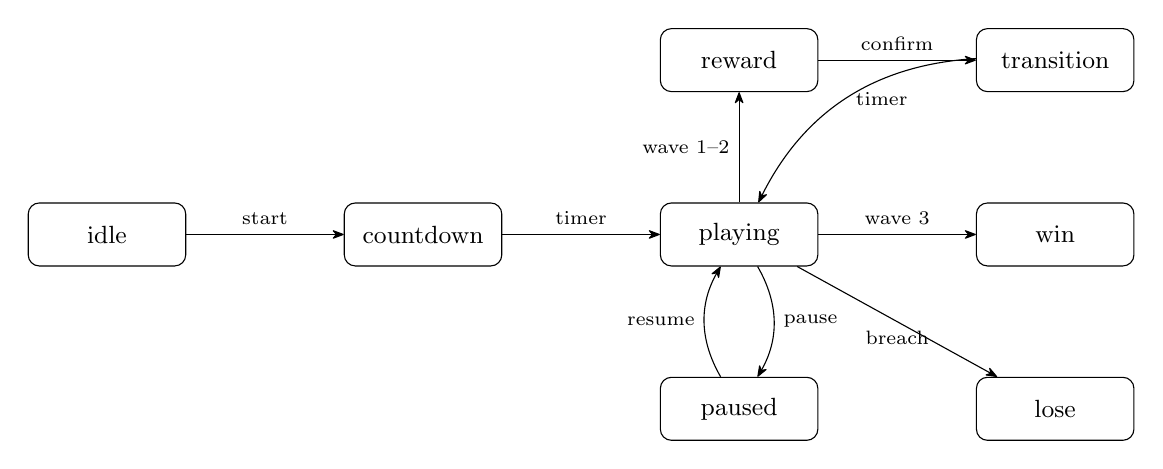
\begin{tikzpicture}[
  >={Stealth[round]}, node distance=14mm and 20mm,
  state/.style={draw, rounded corners, minimum width=20mm, minimum height=8mm,
                font=\small, align=center}, font=\small]
  \node[state] (idle) {idle};
  \node[state, right=of idle] (count) {countdown};
  \node[state, right=of count] (play) {playing};
  \node[state, below=of play] (pause) {paused};
  \node[state, above=of play] (reward) {reward};
  \node[state, right=of reward] (trans) {transition};
  \node[state, right=of play] (win) {win};
  \node[state, below=of win] (lose) {lose};

  \draw[->] (idle) -- node[above,font=\scriptsize]{start} (count);
  \draw[->] (count) -- node[above,font=\scriptsize]{timer} (play);
  \draw[->] (play) to[bend left] node[right,font=\scriptsize]{pause} (pause);
  \draw[->] (pause) to[bend left] node[left,font=\scriptsize]{resume} (play);
  \draw[->] (play) -- node[left,font=\scriptsize]{wave 1--2} (reward);
  \draw[->] (reward) -- node[above,font=\scriptsize]{confirm} (trans);
  \draw[->] (trans) to[bend right] node[right,font=\scriptsize]{timer} (play);
  \draw[->] (play) -- node[above,font=\scriptsize]{wave 3} (win);
  \draw[->] (play) -- node[below,font=\scriptsize]{breach} (lose);
\end{tikzpicture}
\caption{Game states and events.}
\label{fig:states}
\end{figure}

\subsection{Battlefield Layout and Coordinate System}

The battlefield is laid out along a single action axis. The house front stands
on the left at $x=-20$ world units; a narrow strip holds the cannon at $x=-16$;
the green yard the monsters cross runs from $x=-11$ to the spawn line at $x=26$;
and the depth axis $z$ spans 32 units, the width across which the house front
faces the field. Monsters spawn on the right and advance left toward the house.
We made the house front span the full depth, and gave each monster a slightly
different lateral path, so that monsters spread across the field instead of
funnelling into a single point. Only clicks inside the yard are valid targets;
the cannon strip and the house are outside it. Figure~\ref{fig:field} shows the
layout from above.

\begin{figure}[h]
\centering
\resizebox{\linewidth}{!}{%
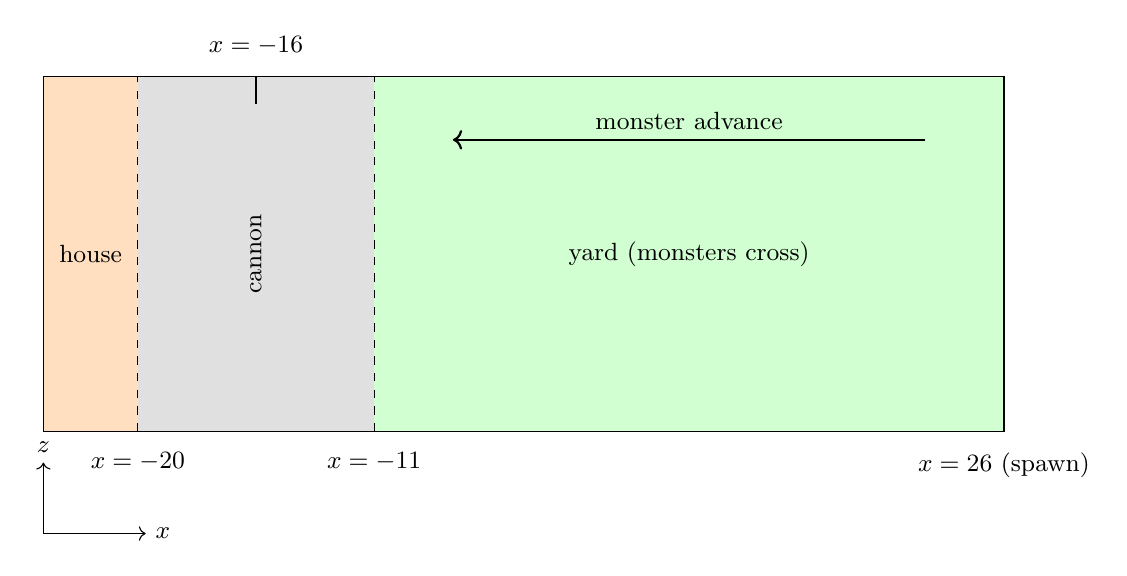
\begin{tikzpicture}[font=\small, every node/.style={font=\small}]
  % zones (schematic; widths exaggerated so the tick labels have room)
  \fill[orange!25] (-1.2,0) rectangle (0,4.5);   % house (left of x=-20)
  \fill[black!12]  (0,0)    rectangle (3,4.5);   % weapon strip (-20..-11)
  \fill[green!18]  (3,0)    rectangle (11,4.5);  % yard (-11..26)
  \draw (-1.2,0) rectangle (11,4.5);
  % zone boundaries
  \draw[dashed] (0,0) -- (0,4.5);   % x=-20  house / strip
  \draw[dashed] (3,0) -- (3,4.5);   % x=-11  strip / yard
  % cannon position (x=-16): short tick at the top, no full line through the text
  \draw (1.5,4.5) -- (1.5,4.15);
  % zone labels
  \node at (-0.6,2.25) {house};
  \node[rotate=90] at (1.5,2.25) {cannon};
  \node at (7,2.25) {yard (monsters cross)};
  % x tick labels (well spaced along the bottom)
  \node[below] at (0,-0.15)  {$x=-20$};
  \node[below] at (3,-0.15)  {$x=-11$};
  \node[below] at (11,-0.15) {$x=26$ (spawn)};
  \node[above] at (1.5,4.65)  {$x=-16$};
  % monster advance arrow (upper yard)
  \draw[->,thick] (10,3.7) -- (4,3.7) node[midway,above]{monster advance};
  % coordinate key, kept clear of the tick labels in the lower-left
  \draw[->] (-1.2,-1.3) -- (0.1,-1.3) node[right]{$x$};
  \draw[->] (-1.2,-1.3) -- (-1.2,-0.4) node[above]{$z$};
\end{tikzpicture}%
}
\caption{Top-down battlefield layout.}
\label{fig:field}
\end{figure}

\subsection{Enemy Design}

There are three enemy classes, designed to trade health against speed so that
the player must decide which monsters to hit first. The easy class is fragile
but fast, the hard class is tough but slow, and the medium class sits between
them. Speed is defined indirectly: each class is given a time to cross the whole
field, from which a constant speed is derived. Table~\ref{tab:enemies} lists the values used in the build. 

\begin{table}[h]
\centering
\caption{Enemy classes and their balance}
\label{tab:enemies}
\begin{tabular}{|p{2.6cm}|p{2.4cm}|p{3.2cm}|p{3.0cm}|}
\hline
Class & Health & Time to cross field & Relative speed \\
\hline
Easy   & 100 & 25 seconds & Fastest \\
\hline
Medium & 200 & 30 seconds & Medium \\
\hline
Hard   & 400 & 35 seconds & Slowest \\
\hline
\end{tabular}
\end{table}

\subsection{Weapon Design and Progression}

The player starts with the Basic weapon and unlocks a stronger one after each of
the first two waves. Each tier deals more damage but reloads more slowly, so the
progression is a reward rather than a free upgrade. Every weapon also charges a
periodic stronger shot, the Big Shot, after a fixed number of normal shots, and
the Advanced weapon fires two projectiles at once. We made one deliberate change
from the original specification: instead of forcing the new weapon on the
player, we let the player choose whether to adopt it, which we found made the
reward feel earned rather than imposed. Table~\ref{tab:weapons} gives the tuning
used in the build.

\begin{table}[h]
\centering
\caption{Weapon tuning.}
\label{tab:weapons}
\begin{tabular}{|p{2.2cm}|p{1.6cm}|p{2.4cm}|p{1.8cm}|p{1.6cm}|p{2.0cm}|}
\hline
Weapon & Damage & Big Shot & Shots & Reload & Unlock \\
\hline
Basic    & 80  & 100 every 3 & 1 & 2 s & start \\
\hline
Medium   & 100 & 120 every 4 & 1 & 2 s & after wave 1 \\
\hline
Advanced & 150 & 170 every 5 & 2 & 3 s & after wave 2 \\
\hline
\end{tabular}
\end{table}

The Basic weapon also has the slowest projectile and the Advanced the fastest,
so higher tiers both hit harder and land sooner.

\subsection{Shooting and Area-of-Effect Damage Model}

A click chooses a target point on the ground; the cannon fires a projectile that
arcs to that point and, on landing, damages every enemy within a fixed blast
radius. We chose area damage rather than single-target hits because a defence
game is about crowds: a well-placed shot should reward the player for catching
several monsters at once. Damage falls off linearly with distance from the
impact point. With $d$ the distance from the impact to an enemy, $R$ the blast
radius (6 world units in the build), and $D$ the weapon damage, the damage dealt
is

\begin{equation}
\text{damage}(d) =
\begin{cases}
D\left(1 - \dfrac{d}{R}\right), & 0 \le d \le R, \\[2mm]
0, & d > R.
\end{cases}
\end{equation}

An enemy at the exact impact point takes the full weapon damage; one at the edge
of the radius takes almost none; one outside takes nothing.
Figure~\ref{fig:falloff} plots this falloff.

\begin{figure}[h]
\centering
\begin{tikzpicture}[font=\small]
  \draw[->] (0,0) -- (6.4,0) node[right]{$d$ (distance)};
  \draw[->] (0,0) -- (0,3.2) node[above]{damage};
  \draw[thick] (0,3) -- (6,0);
  \draw[dashed] (0,3) -- (-0.0,3);
  \node[left] at (0,3) {$D$};
  \node[below] at (6,0) {$R$};
  \node[below left] at (0,0) {$0$};
  \draw[dashed] (6,0) -- (6,-0.05);
\end{tikzpicture}
\caption{Linear area-of-effect damage falloff.}
\label{fig:falloff}
\end{figure}

\subsection{Wave Design and Difficulty Progression}

The game has three waves with a fixed, escalating roster. Each wave adds tougher monsters
than the last, as shown in Table~\ref{tab:waves}. Within a wave, monsters spawn
one at a time on a schedule set by their class --- the tougher the class, the
longer the gap before it appears --- and the first monster of each wave arrives
three seconds after the countdown ends. Table~\ref{tab:spawn} gives the
intervals.

\begin{table}[h]
\centering
\caption{Wave composition}
\label{tab:waves}
\begin{tabular}{|c|c|c|c|c|}
\hline
Wave & Easy & Medium & Hard & Total \\
\hline
1 & 2 & 1 & 0 & 3 \\
\hline
2 & 2 & 2 & 1 & 5 \\
\hline
3 & 2 & 2 & 3 & 7 \\
\hline
\end{tabular}
\end{table}

\begin{table}[h]
\centering
\caption{Spawn interval per class}
\label{tab:spawn}
\begin{tabular}{|c|c|}
\hline
Class & Interval \\
\hline
Easy   & 3 seconds \\
\hline
Medium & 4 seconds \\
\hline
Hard   & 5 seconds \\
\hline
\end{tabular}
\end{table}

\subsection{Victory and Defeat Conditions}

Defeat is positional, not health-based: the game is lost the instant any monster
reaches the house front, regardless of how many monsters remain or how much
health they have. We chose this because it makes the player's job clear --- stop
everything from getting through --- and keeps the stakes high. Victory is the
opposite: the player must clear every monster of the third wave, with none left
on the field.

\section{User Experience and Interface Design}

This section covers how the player perceives and controls the game.

\subsection{Screen Flow}

The player enters on a welcome screen, where they may type a name (used for the
leaderboard) or start anonymously, and may view the leaderboard. Play leads to
either a win or a lose screen, both of which show the leaderboard and offer a way
back --- restart for another attempt, or return to the welcome screen.
Figure~\ref{fig:flow} shows the flow.

\begin{figure}[h]
\centering
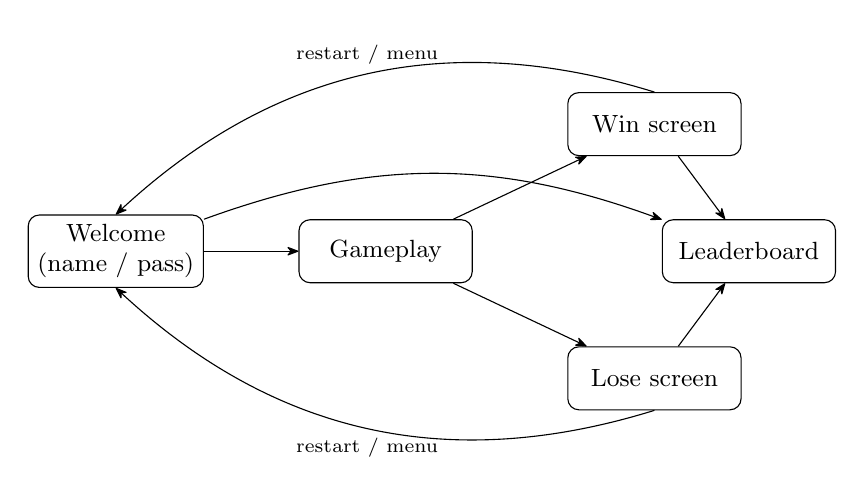
\begin{tikzpicture}[
  >={Stealth[round]}, node distance=8mm and 12mm,
  box/.style={draw, rounded corners, minimum width=22mm, minimum height=8mm,
              align=center, font=\small}, font=\small]
  \node[box] (start) {Welcome\\(name / pass)};
  \node[box, right=of start] (play) {Gameplay};
  \node[box, above right=of play] (win) {Win screen};
  \node[box, below right=of play] (lose) {Lose screen};
  \node[box, right=24mm of play] (board) {Leaderboard};
  \draw[->] (start) -- (play);
  \draw[->] (play) -- (win);
  \draw[->] (play) -- (lose);
  \draw[->] (win) -- (board);
  \draw[->] (lose) -- (board);
  \draw[->] (start) to[bend left=20] (board);
  \draw[->] (win.north) to[bend right=30] node[above,font=\scriptsize]{restart / menu} (start.north);
  \draw[->] (lose.south) to[bend left=30] node[below,font=\scriptsize]{restart / menu} (start.south);
\end{tikzpicture}
\caption{Screen flow.}
\label{fig:flow}
\end{figure}

\subsection{HUD and Overlays}

During play, a heads-up display keeps the current wave number and elapsed time
in view, together with a picker for switching between unlocked weapons. Short
overlays handle the moments between action: the pre-play countdown, the pause
screen, the between-wave reward and transition messages, and the final win or
lose screen. The overlays pause the simulation so no monster slips through while
the player reads them.

\subsection{Visual Feedback Design}

Every action gives the player an immediate, legible cue. The clicked target is
marked with an X on the ground; each monster carries a health bar that shrinks
and shifts colour as it takes damage; a monster that is hit flashes red; and a
landing shot produces a burst at the impact point, larger for a Big Shot. We
treat this feedback as a usability requirement, not decoration: without it the
player cannot tell whether a shot connected.

\section{Leaderboard and Ranking Design}

The leaderboard turns a finished game into a comparable record. A run is
described by the player's name, the total time taken, the furthest wave reached,
and whether all three waves were cleared. The ranking has to be fair to two
different kinds of player: those who finished the game and those who did not. We
order players who cleared the game above those who did not; among the winners,
the faster time ranks higher; among the rest, the player who reached a deeper
wave ranks higher, with more recent attempts shown first. Table~\ref{tab:rank}
states this as the ordered list of sort keys, which is exactly how the database
returns the board.

\begin{table}[h]
\centering
\caption{Ranking sort keys, in order of priority}
\label{tab:rank}
\begin{tabular}{|c|p{6.0cm}|p{3.2cm}|}
\hline
Order & Sort key & Direction \\
\hline
1 & Cleared the game (won) & Winners first \\
\hline
2 & Furthest wave reached & Higher first \\
\hline
3 & Completion time (winners only) & Faster first \\
\hline
4 & When the run was recorded & More recent first \\
\hline
\end{tabular}
\end{table}

\section{From Design to Specification}

The decisions above are recorded formally and in full in the Software
Requirements Specification, where each requirement
carries an acceptance criterion. The next chapter turns this design into a
working application and refers back to these identifiers as it goes, so that the
finished system can be checked against the specification in
Chapter~\ref{ch:results}.

% ===========================================================================
\chapter{Materials and Methods}\label{ch:methods}
% ===========================================================================

This chapter describes how we turned the design of Chapter~\ref{ch:design} into
a working application. For each part we state what it is and why we chose it,
then show how it works in enough detail that the craft can be checked. The whole
system is a single Next.js project that contains both the browser client and the
small server behind the leaderboard.

\section{Technology Stack and Rationale}

We built the game on a small, modern web stack, summarised in
Table~\ref{tab:stack}. Two choices are worth singling out. First, we used
Three.js directly rather than a React wrapper such as react-three-fiber, because
we wanted to own the render loop ourselves and learn the graphics first-hand
rather than through an abstraction. Second, we used the Next.js App Router so
that one project serves the client and also exposes the leaderboard endpoints,
leaving no separate backend to deploy.

\begin{table}[htbp]
\centering
\caption{Technology stack and rationale}
\label{tab:stack}
\begin{tabular}{|p{2.6cm}|p{1.2cm}|p{4.0cm}|p{4.2cm}|}
\hline
Technology & Version & Role & Why this choice \\
\hline
Next.js & 16 & App framework: routing and the server route handlers &
One framework for the client and the small backend \\
\hline
React & 19 & Component UI for menus, HUD and overlays &
Familiar component model; pairs with our own store \\
\hline
TypeScript & 5 & Static typing across the whole codebase &
Catches errors at compile time and documents the data shapes \\
\hline
Three.js & 0.184 & WebGL 3D rendering of the scene &
Direct control of the scene graph and the render loop \\
\hline
Tailwind CSS & 4 & Styling the two-dimensional interface &
Consistent styling without separate stylesheet files \\
\hline
better-sqlite3 & 12 & Server-side leaderboard storage &
A zero-configuration embedded database with a synchronous API \\
\hline
\end{tabular}
\end{table}

\section{System Architecture}

The application obeys one organising idea: a single object holds the whole game
world, and everything else either reads it or produces a new version of it. This
gives a four-layer architecture with a strictly one-directional data flow, which
we describe here before the details.

\subsection{Layered Architecture Overview}

We separate the code into four layers, shown in Figure~\ref{fig:layers}. The UI
layer is the React components the player sees. The state-management layer holds
the single game state and the reducer that updates it. The systems layer is the
gameplay logic that reads the state and decides what should change. The
rendering layer draws the state with Three.js. The rule we keep is that
dependencies only point downward: the UI and systems depend on the state, the
renderer depends on the state, but the state depends on nothing. Keeping the
reducer free of React and Three.js means we can reason about, and test, the game
logic on its own.

\begin{figure}[htbp]
\centering
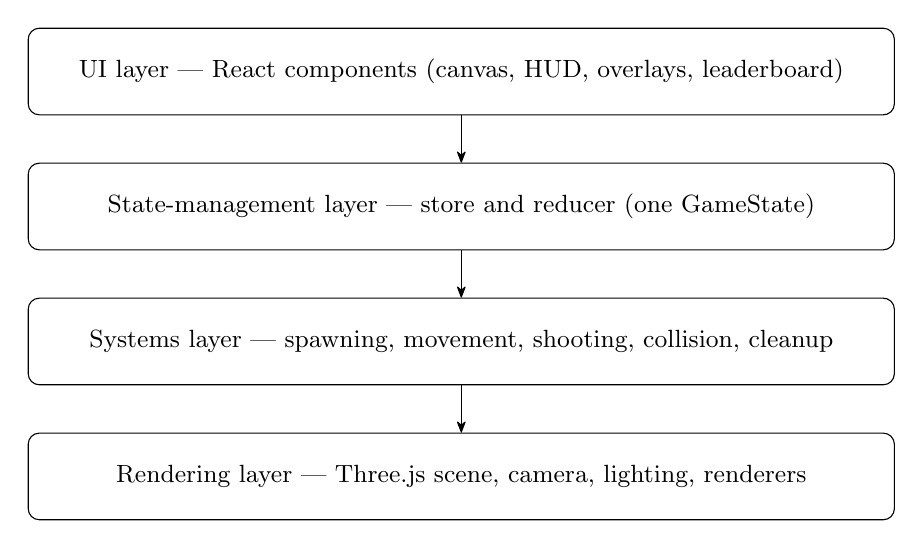
\begin{tikzpicture}[font=\small, node distance=6mm, >={Stealth[round]},
  layer/.style={draw, rounded corners, minimum width=11cm, minimum height=11mm,
                align=center}]
  \node[layer] (ui) {UI layer --- React components (canvas, HUD, overlays, leaderboard)};
  \node[layer, below=of ui] (state) {State-management layer --- store and reducer (one GameState)};
  \node[layer, below=of state] (sys) {Systems layer --- spawning, movement, shooting, collision, cleanup};
  \node[layer, below=of sys] (rend) {Rendering layer --- Three.js scene, camera, lighting, renderers};
  \draw[->] (ui) -- (state);
  \draw[->] (state) -- (sys);
  \draw[->] (sys) -- (rend);
\end{tikzpicture}
\caption{Layered Architecture.}
\label{fig:layers}
\end{figure}

\subsection{Project Structure and Module Organisation}

The source tree mirrors these layers, so that the location of a file tells the
reader its job. Every file also begins with a header comment stating its single
responsibility and what does not belong in it, which keeps modules focused. The
layout is shown below.

\begin{verbatim}
src/
  app/        Next.js routes and the /api/scores backend
  core/       store, reducer, game loop, constants, weapons, event bus
  systems/    gameplay logic (spawn, movement, shooting, collision, cleanup)
  entities/   plain-data factories (Enemy, Bullet, House, HealthBar, ...)
  lib/        Three.js setup, camera, lighting, models, raycasting, db
  components/ React UI (GameCanvas, HUD, overlays, Leaderboard)
  hooks/      the React-to-store bridge and score submission
  types/      shared TypeScript types (game, actions, entity, score)
\end{verbatim}

\subsection{Data Flow: Input to Render}

Every change follows the same path, shown in Figure~\ref{fig:dataflow}. An input
(a click, or simply the next animation frame) is turned into an action; the
action is dispatched to the reducer; the reducer returns a new game state; the
systems run against that state and may dispatch further actions; and finally the
renderer draws the latest state. Because this path is the same everywhere,
behaviour is predictable and easy to trace.

\begin{figure}[H]
\centering
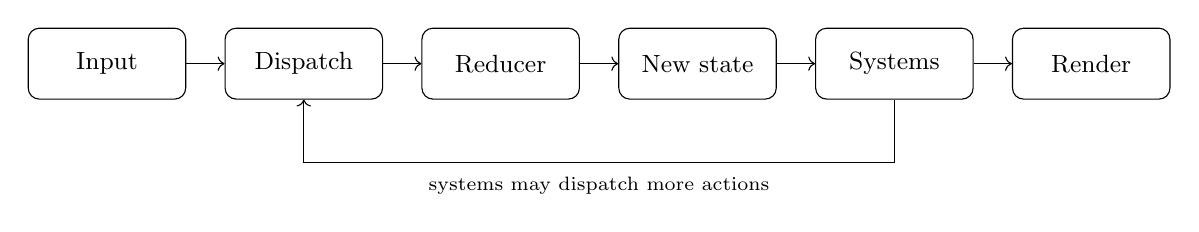
\begin{tikzpicture}[
  box/.style={draw, rounded corners, minimum height=9mm, minimum width=20mm,
              align=center, font=\small}]
  % six steps placed by absolute coordinates (no positioning library needed)
  \node[box] (in)   at (0,0)    {Input};
  \node[box] (disp) at (2.5,0)  {Dispatch};
  \node[box] (red)  at (5,0)    {Reducer};
  \node[box] (st)   at (7.5,0)  {New state};
  \node[box] (sys)  at (10,0)   {Systems};
  \node[box] (ren)  at (12.5,0) {Render};
  % forward arrows (default tikz arrow tip; no arrows.meta needed)
  \draw[->] (in)   -- (disp);
  \draw[->] (disp) -- (red);
  \draw[->] (red)  -- (st);
  \draw[->] (st)   -- (sys);
  \draw[->] (sys)  -- (ren);
  % feedback loop: systems may dispatch more actions
  \draw[->] (sys.south) -- ++(0,-0.8) -| (disp.south);
  \node[font=\scriptsize] at (6.25,-1.55) {systems may dispatch more actions};
\end{tikzpicture}
\caption{The per-frame data flow.}
\label{fig:dataflow}
\end{figure}


\section{State Management}\label{sec:state}

A real-time game changes state many times a second, so how that state is held
and updated is the heart of the implementation.

\subsection{The GameState Model}

The whole world is one TypeScript object. Defining it as an interface makes the
contract explicit: the reducer must return a valid one, the systems receive and
return one, and the interface is the single source of truth. Its shape is shown
below.

\begin{verbatim}
interface GameState {
  status: "idle" | "countdown" | "playing" | "paused"
        | "reward" | "transition" | "win" | "lose";
  wave: number;  weapon: WeaponLevel;  weaponsUnlocked: WeaponLevel[];
  attackCount: number;  weaponCooldown: number;   // Big Shot + reload
  elapsed: number;  countdown: number;  waveTransition: number;
  player: { hp: number };
  enemies: Enemy[];  bullets: Bullet[];
  marker: TargetMarker | null;  playerName: string | null;
}
\end{verbatim}

\subsection{Reducer and Action Set}

Every change to the state goes through one pure function of the form
\texttt{(state, action) $\to$ state}. It has no side effects: it never touches
the network, the DOM or Three.js, it only computes the next world from the
current one. Limiting changes to a closed set of actions means the whole
behaviour can be read in one place, and any change can be logged and replayed.
Table~\ref{tab:actions} lists the main actions and what each does. The reducer
also enforces rules through guards: a shot is ignored while the weapon is still
reloading, and the game flips to the lost state the moment a moving enemy reaches
the house line.

\begin{table}[htbp]
\centering
\caption{The main actions and their effect on the state}
\label{tab:actions}
\begin{tabular}{|p{3.6cm}|p{9.0cm}|}
\hline
Action & Effect on the game state \\
\hline
START\_GAME & Resets to a fresh world in the countdown state; keeps the entered name \\
\hline
TICK & Advances the countdown, elapsed time and reload timer by the frame's $dt$ \\
\hline
SPAWN\_ENEMY / MOVE\_ENEMIES & Adds a new enemy; advances all enemies and checks for a breach \\
\hline
FIRE\_SHOT & Builds the active weapon's projectile(s), advances the Big Shot counter, starts the reload \\
\hline
DAMAGE\_ENEMY & Reduces one enemy's health and marks it dead at zero \\
\hline
WAVE\_CLEARED / RESOLVE\_REWARD & Unlocks the next weapon, then runs the between-wave transition \\
\hline
PAUSE / RESUME & Freezes and resumes the simulation \\
\hline
WIN / LOSE & Moves to a terminal state and stops the simulation \\
\hline
\end{tabular}
\end{table}



\section{The Game Loop}

The game loop is what makes the world advance over time. We keep it deliberately
thin and separate from the gameplay it drives.

\subsection{The Driver and Delta-Time Clamping}

The driver is a minimal wrapper around the browser's
\texttt{requestAnimationFrame}. Each frame it measures the time since the last
frame, in seconds, and hands that delta-time to one callback. We clamp the delta
to a maximum of one fifteenth of a second: if the browser tab is in the
background and then returns, the gap between frames can be huge, and without the
clamp the simulation would jump forward in a single step. Clamping turns that
jump into a slightly slow frame instead. The driver knows only when to step; it
has no idea what a step does, which keeps it reusable and trivial to reason
about.

\subsection{Per-Frame Orchestration}

The callback is where one frame's work is sequenced, and it follows the data
flow of Figure~\ref{fig:dataflow}. In order, it dispatches \texttt{TICK} to
advance the timers; updates the spawn scheduler so the wave's enemies appear on
time; advances the enemies and the bullets; detects any bullet that has just
reached its target and broadcasts its impact once; checks whether the wave is
complete; and finally renders the scene. Crucially, the gameplay steps run only
while the game is in the playing state, and the renderer is fed a delta-time of
zero when the game is not playing, so that on pause, win or lose the scene is
still drawn but nothing moves.

\section{Gameplay Systems}

The systems layer holds the gameplay logic. Each system is an independent module
that reads the current state and produces actions, never touching React or
Three.js. We describe each in turn, with the mechanism it uses.

\subsection{Spawning and Wave Scheduling}

The spawn scheduler is a small stateful object that releases the current wave's
roster over time. It keeps the list of enemy types for the wave, a cursor for how
many have appeared, and a timer counting down to the next one. The first enemy
arrives three seconds after the countdown, and the gap before each subsequent
enemy is that enemy's own interval, so tougher classes appear less often. Once
the cursor reaches the end of the roster it stops, and it reports the roster as
complete so the loop can detect a cleared wave. The scheduler advances only while
the game is playing, so it freezes cleanly on pause and re-arms for a new game.

\subsection{Enemy State Machine and Movement}

Each enemy follows a three-state lifecycle, shown in Figure~\ref{fig:enemystate}:
it is born spawning, flips to moving on its first update, and becomes dead when
its health reaches zero. Only moving enemies advance. We define each class by the
time it should take to cross the whole field and derive a constant speed from
that distance, so the balance is independent of the field size. To stop enemies
walking in a straight line and bunching up, each one weaves along a smooth sine
path of its own random width and phase around its spawn lane. Movement clamps an
enemy at the house line; the reducer treats a moving enemy that has reached that
line as a breach and ends the game.

\begin{figure}[htbp]
\centering
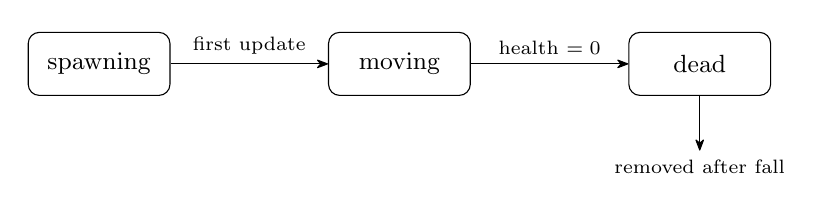
\begin{tikzpicture}[font=\small, node distance=20mm, >={Stealth[round]},
  st/.style={draw, rounded corners, minimum width=18mm, minimum height=8mm}]
  \node[st] (sp) {spawning};
  \node[st, right=of sp] (mv) {moving};
  \node[st, right=of mv] (dd) {dead};
  \draw[->] (sp) -- node[above,font=\scriptsize]{first update} (mv);
  \draw[->] (mv) -- node[above,font=\scriptsize]{health $=0$} (dd);
  \draw[->] (dd) -- ++(0,-1.1) node[below,font=\scriptsize]{removed after fall};
\end{tikzpicture}
\caption{The enemy lifecycle. A moving enemy that takes damage stays moving
until its health reaches zero.}
\label{fig:enemystate}
\end{figure}

\subsection{The Shooting Pipeline and Event Bus}

A shot begins as a click on the canvas. We cast a ray from the camera through the
cursor onto the mathematical ground plane to get a world point, then check that
the point lies inside the yard; clicks outside it are ignored. A valid click does
not change state directly. Instead it emits a \texttt{shoot:requested} event on a
small typed event bus, and a handler turns that event into a \texttt{FIRE\_SHOT}
action. We route it through an event bus because a shot is a momentary
notification, not part of the state: keeping such one-off events out of the
reducer stops it from having to remember what it has already handled, and lets
the input code stay independent of the reducer.

\subsection{Projectile Physics}

A projectile leaves the cannon muzzle and must land exactly on the clicked point
after a weapon-dependent flight time $T$, while following an arc rather than a
straight line. We use classic projectile motion,

\begin{equation}
p(t) = p_0 + v\,t + \tfrac{1}{2}\,g\,t^2,
\end{equation}

where $p_0$ is the muzzle and $g$ is a constant downward gravity. The horizontal
velocities are fixed to cover the gap over the flight, $v_x=(x_T-x_0)/T$ and
$v_z=(z_T-z_0)/T$, and the vertical launch velocity is solved from the landing
condition, $v_y=(y_T-y_0-\tfrac12 g T^2)/T$, so the bullet always arrives on
target at $t=T$ regardless of distance. After landing it rests on the target for
a short linger before it is removed.

\subsection{Collision and Area-of-Effect Resolution}

The first frame a bullet reaches its target, the loop broadcasts a single impact
event; a set of already-impacted bullet identifiers guards against resolving the
same blast twice on later frames. Resolving the impact is a pure function: for
every living enemy within the blast radius it returns the falloff damage
$D(1-d/R)$ derived in Chapter~\ref{ch:design}, and the loop dispatches one
\texttt{DAMAGE\_ENEMY} action per hit. Dead enemies are skipped, so a destroyed
monster no longer takes part in collisions.

\subsection{Entity Cleanup}

Inactive entities are removed so they stop consuming updates and draw calls. A
bullet is dropped once its flight time plus linger has elapsed. A dead enemy
stays in the state briefly so the renderer can play its falling animation; when
that animation finishes, the renderer asks the store to remove it. Keeping the
removal driven by the animation avoids a monster vanishing mid-fall.

\section{Rendering Layer}

The rendering layer turns the game state into pixels with Three.js and WebGL.
Its guiding principle is that the renderer is a mirror of the state, never a
second source of truth: it owns Three.js meshes, but the meaning of the world
lives only in the state.

\subsection{Scene, Camera, and Lighting}

On entering the game we build the Three.js context once: a WebGL renderer with
antialiasing, a capped pixel ratio and soft shadow maps; a scene with a plain
background and no fog, so the whole yard stays evenly lit; a perspective camera
placed high and behind the near edge, looking down so the field is framed from
above; and the lighting, an ambient light for overall visibility plus a single
directional light that acts as the sun and casts the shadows. The static scenery
--- ground, yard, strip and fence --- is added once at this point and never
rebuilt.

\subsection{Asset Pipeline: Model Loading and Caching}

Every 3D model is listed in one manifest that maps a logical key to a file under
the public folder, summarised in Table~\ref{tab:models}. Loading a model is
asynchronous and costly, so we preload them all once when the game route opens,
keep the parsed result in memory, and from then on hand out clones synchronously.
This avoids both a per-spawn network request and the visible pop-in of a model
appearing late. Because the enemies are skinned, animated models, we clone them
with a skeleton-aware clone so each instance gets its own bones; a missing file
is skipped with a warning rather than crashing the game.

\begin{table}[htbp]
\centering
\caption{Model files and the entities they represent}
\label{tab:models}
\begin{tabular}{|p{5.5cm}|p{6.5cm}|}
\hline
Model file & In-game entity \\
\hline
house.glb & The protected house \\
\hline
fence.glb & A perimeter fence segment, tiled around the field \\
\hline
enemy-easy / medium / hard.glb & The three enemy classes \\
\hline
weapon-basic / medium / advanced.glb & The three cannon tiers \\
\hline
\end{tabular}
\end{table}

\subsection{Renderer--State Reconciliation}

Each renderer keeps a map from entity identifier to live mesh and, once per
frame, reconciles that map against the latest state array. New entities get a
fresh mesh added to the scene; surviving ones have their position and rotation
updated; entities no longer in the state have their mesh removed and disposed.
This is a small version of the same reconciliation idea React uses for the DOM,
and it is what lets the rest of the code treat the state, not the scene, as the
truth.

\subsection{Animation, Health Bars, and Effects}

On top of the meshes, the renderer drives the things that make the action
legible: an animation mixer plays each enemy's walk and death clips; a health bar
floats above every enemy, always facing the camera, shrinking and shifting from
green to red as health drops; a hit flash tints a damaged enemy; and a burst
appears at each impact, larger for a Big Shot. All of these advance by the
frame's delta-time, so feeding them a delta of zero when the game is not playing
freezes them along with the rest of the simulation.

\subsection{Raycasting and Target Picking}

Target picking converts a screen click into a world point. We translate the
canvas-relative click into normalised device coordinates, build a camera ray
from them, and intersect that ray with the ground plane $y=0$ --- a plane, not a
mesh, so the hit is exact and independent of the visible floor. The resulting
point is then accepted only if it falls inside the yard, which is how
out-of-bounds clicks are rejected before any shot is fired.

\section{The Leaderboard Subsystem}

The leaderboard is the one place the project crosses from the browser to a
server. It is a compact full-stack slice: we own the data model, the HTTP
contract, the server-side validation, the ranking query, and the client that
talks to it.

\subsection{Data Model and Persistence}

A finished run is stored as one row in a \texttt{scores} table, shown in
Table~\ref{tab:schema}. We use SQLite through better-sqlite3 because it needs no
separate database server and its synchronous API fits the request handlers
naturally. One module is the only code that touches the database; it owns the
file, the table and the prepared statements, so the storage engine could be
swapped behind it without changing anything else. In development the framework
reloads modules on every edit, so we cache the open connection on a global to
avoid leaking file handles across reloads.

\begin{table}[htbp]
\centering
\caption{The \texttt{scores} table}
\label{tab:schema}
\begin{tabular}{|p{3.4cm}|p{2.6cm}|p{6.0cm}|}
\hline
Column & Type & Meaning \\
\hline
id & integer & Auto-increment primary key \\
\hline
name & text & The player's display name \\
\hline
time\_ms & integer & Total play time in milliseconds (lower is faster) \\
\hline
wave\_reached & integer & Furthest wave reached, 1 to 3 \\
\hline
won & integer & 1 if all three waves were cleared, else 0 \\
\hline
created\_at & integer & When the run was recorded (epoch milliseconds) \\
\hline
\end{tabular}
\end{table}

\subsection{HTTP API Design}

The client reaches the database only through two endpoints, listed in
Table~\ref{tab:api}, written as Next.js route handlers. They run on the Node
runtime rather than the edge runtime because better-sqlite3 is a native module.
The contract is small and typed: one operation records a run, the other returns
the ranked list.

\begin{table}[htbp]
\centering
\caption{The leaderboard HTTP API}
\label{tab:api}
\begin{tabular}{|p{1.4cm}|p{3.2cm}|p{7.4cm}|}
\hline
Method & Path & Purpose \\
\hline
GET & /api/scores?limit=N & Return the top $N$ runs, already ranked \\
\hline
POST & /api/scores & Record one finished run and return it with its rank \\
\hline
\end{tabular}
\end{table}

\subsection{Server-Side Validation}

The server never trusts the request body. Before storing a run it checks that
the name is a non-empty string, trims it and caps it at twenty characters; that
the time is a positive number; that the wave is an integer from one to three;
and that the won flag is a boolean. Anything malformed is rejected with a
client-error response, so only well-formed runs ever reach the table.

\subsection{The Ranking Query}

The ranking rules from Chapter~\ref{ch:design} are expressed in a single
\texttt{ORDER BY} clause, so the database returns the board already sorted:

\begin{verbatim}
ORDER BY won          DESC,                       -- winners first
         wave_reached DESC,                       -- then deepest progress
         CASE WHEN won = 1 THEN time_ms END ASC,  -- winners: fastest first
         created_at   DESC                        -- the rest: most recent first
\end{verbatim}

Doing the ranking in the query keeps the client simple: it receives rows in
final order and only assigns each a position number.

\subsection{Client Integration}

On the browser side, thin typed wrappers around \texttt{fetch} hide the URLs and
JSON handling, so a component just awaits the ranked list or posts a run. A run
is recorded exactly once, at the moment the game reaches win or lose, and only
for named sessions; anonymous runs are skipped. Because the end screens mount and
unmount, and React may invoke effects twice in development, we centralise the
submission in one always-mounted provider with a guard, which guarantees a single
record per game. The provider exposes the stored entry so the end screen can
highlight the player's new row, and the leaderboard view shows clear loading,
empty and error states.

\section{Engineering Practices}

A few practices run across the whole codebase and are worth noting on their own.

\subsection{Type Safety with TypeScript}

The same TypeScript types describe the data everywhere it travels: the game
state, the closed set of actions, the entities and the leaderboard entry, the
last of which is shared by both the server and the browser so the HTTP contract
is checked at compile time on both sides. The action set is an exhaustive union,
which means the compiler warns us if the reducer forgets to handle a case. Most
mistakes are caught before the game ever runs.

\subsection{Separation of Concerns and Self-Documenting Modules}

Every module has a single responsibility, and every file opens with a header
stating what it is for and what deliberately does not belong in it. Combined with
the downward-only dependency rule between layers, this keeps modules small and
their boundaries clear, which is what made it possible to write, and to explain,
each system in isolation in this chapter.

\subsection{ Phased Development}

We built the game incrementally rather than all at once. Each phase added one
capability --- the scene, then enemies, then movement, then shooting, then the
combat pipeline, then weapon progression, and finally the leaderboard --- and
each was committed as a working slice. Building in phases meant the game ran at
every step, so a problem could be traced to the small change that introduced it
rather than hidden inside a large one.

% ===========================================================================
\chapter{Results and Discussion}\label{ch:results}
% ===========================================================================

This chapter shows that the finished system works, checks it against the
requirements and the quality targets, and then reflects on the decisions behind
it. The first half presents evidence; the second half interprets it.

\section{Results}

We present the results as objective evidence: how completely the implementation
covers the design, what a full session looks like, the leaderboard in use, and
how the running game measures against the quality targets.

\subsection{Requirement Coverage and Traceability}

The design of Chapter~\ref{ch:design} and the implementation of
Chapter~\ref{ch:methods} were built to line up, subsystem by subsystem.
Table~\ref{tab:trace} traces each subsystem to the modules that realise it and
records its status. Every subsystem is implemented; three were realised with a
deliberate change from the original specification. First, a newly unlocked
weapon is offered to the player to adopt rather than forced on them, which we
found made the reward feel earned. Second, we removed the numeric score from the
heads-up display, because in a defence game the wave and timer already convey
progress and the score added clutter without meaning. Third, we tuned the enemy
crossing times slightly slower than first specified, after play-testing showed
the original pace left too little time to react.

\begin{table}[htbp]
\centering
\caption{Requirement coverage: subsystem to implementing modules}
\label{tab:trace}
\begin{tabular}{|p{4.0cm}|p{5.6cm}|p{2.8cm}|}
\hline
Subsystem (Ch.~\ref{ch:design}) & Implementing modules (Ch.~\ref{ch:methods}) & Status \\
\hline
Game session and lifecycle & reducer state machine, game loop & Implemented \\
\hline
Battlefield environment & scenery, world constants & Implemented \\
\hline
Enemy system & enemy factory, spawn and movement systems & Implemented \\
\hline
Weapon system & weapon table, fire-shot reducer & Changed \\
\hline
Shooting and damage & raycasting, shooting pipeline, collision & Implemented \\
\hline
Wave progression & spawn scheduler, wave-clear handling & Implemented \\
\hline
Runtime control & reducer guards, loop gating & Implemented \\
\hline
Victory and defeat & reducer end-state transitions & Implemented \\
\hline
Heads-up display and overlays & HUD and overlay components & Changed \\
\hline
Rendering & Three.js setup, renderers, lighting, camera & Implemented \\
\hline
Physics and collision & bullet, collision and cleanup systems & Implemented \\
\hline
Leaderboard and ranking & database, API route, client and submit hook & Implemented \\
\hline
\end{tabular}
\end{table}

\subsection{Gameplay Walkthrough}

A complete session runs from the welcome screen, through the countdown and three
waves of combat, to a win or lose screen. We successfully navigate the welcome screen with the name entry, the countdown,
mid-wave combat with several monsters advancing and health bars above them, a Big
Shot landing with its larger burst, the between-wave reward where a new weapon is
offered, and the final victory screen.



\subsection{The Leaderboard in Action}

The leaderboard after several runs. Players who
cleared all three waves appear first, ordered by their completion time; players
who did not finish follow, grouped by the furthest wave they reached. When the
board is shown on an end screen, the player's own most recent run is highlighted.



\subsection{Performance Evaluation}

We measured the running game in Google Chrome on a desktop machine. The scene
loaded in about two seconds, and during play the frame rate stayed at the
display's 60\,Hz ceiling, dropping only briefly to about 31 in the busiest
combat --- always at or above the 30 FPS target. Table~\ref{tab:perf}
summarises the results.

\begin{table}[htbp]
\centering
\caption{Quality targets and observed results}
\label{tab:perf}
\begin{tabular}{|p{5.2cm}|p{2.6cm}|p{4.2cm}|}
\hline
Metric & Target & Result \\
\hline
Frame rate, normal play & at least 30 FPS & 55--60 FPS (at the 60\,Hz cap) \\
\hline
Frame rate, heaviest combat & at least 30 FPS & 45--55 FPS, brief dips to about 31 \\
\hline
Initial scene load time & under 10 seconds & about 2.1 seconds \\
\hline
\end{tabular}
\end{table}

The brief dips come mainly from garbage collection: the immutable state model
creates many short-lived objects each frame, and reclaiming them pauses the main
thread for a moment. They could be smoothed out by reusing objects instead of
recreating them and by drawing the enemies as instanced meshes; since the frame
rate never fell below the target, we leave these as future optimisations.

\section{Discussion}

We now interpret the results and surface the judgement behind the main
decisions.

\subsection{Analytical Reflections}

Specifying the game before building it paid off: because each behaviour already
had an acceptance criterion, the implementation had a clear target and the
finished system could be checked against it rather than against opinion. Where
reality pushed back, the specification changed for good reasons --- the weapon
choice, the removed score and the slower enemies were all decisions taken during
play-testing, and writing them down kept the design honest about what the game
actually is. The main lesson was that a requirement is only useful if it is
testable; the rules that were easy to verify by playing were the ones that
survived.

\subsection{Technical Reflections}

The architectural bets held up. Building our own state container instead of
adding a library kept the data flow visible and was enough for a single-player
game. Using Three.js directly
rather than a React wrapper gave us full control of the render loop and a
first-hand understanding of the graphics. The strict separation between the layers was the single
most valuable choice: keeping the reducer free of rendering let us reason about
the game logic on its own, which is also what made the implementation chapter
possible to explain system by system. With more time we would add automated
tests around the reducer, which its purity makes straightforward.


\subsection{Limitations}

The system is bounded in ways worth stating plainly. It is a single-player,
desktop, mouse-only experience; there are no user accounts and no cross-device
play. The leaderboard uses a local database file, which is ideal for development
but does not persist on a stateless hosting platform without a hosted database.
And the three waves are fixed rather than
generated. None of these affect the goals of the project, but each is a natural
starting point for future work.

% ===========================================================================
\chapter{Conclusion and Perspective}\label{ch:conclusion}
% ===========================================================================

This final chapter restates what the project achieved against its objectives,
names the skills it demonstrates, and points to where it could go next.

\section{Conclusion}

We set out to build a complete, working, browser-based 3D game that would let us
practise both the analytical work of specifying a system and the technical work
of implementing it. We achieved that. The analytical half produced a full
specification and game design --- the gameplay, the enemy, weapon and wave
balance, the area-of-effect damage model and the leaderboard ranking rules. The
technical half realised that design as a real-time application built with
Next.js, React, TypeScript and Three.js, organised into a clear four-layer
architecture, and backed by a small full-stack slice: an HTTP API over an SQLite
database that records finished runs and returns them ranked. Measured against the
success criteria of Chapter~\ref{ch:objectives}, the game plays through all three
waves, the weapon progression and win and lose conditions behave as designed, and
the leaderboard records and ranks runs correctly.

\section{Skills Demonstrated}

The project demonstrates two complementary skill sets. On the analytical side it
shows requirements elicitation, writing a structured and testable specification,
designing business rules and game balance, mapping out the user experience, and
keeping the whole thing traceable from a rule to the line of code that enforces
it. On the technical side it shows component-based interface design, state
management built from first principles, real-time rendering with WebGL, HTTP API
and database design, and end-to-end type safety with TypeScript. As set out in
the introduction, the technical skills were the ones we practised day-to-day
during the internship, while the analytical work was something we had only
observed there; building this independent project is where we turned that
observation into hands-on practice and brought both together into a single,
demonstrable piece of work.

\section{Future Work}

The system was designed to be extended, and several directions follow naturally
from its architecture. The leaderboard could record richer metrics --- accuracy,
monsters defeated, per-weapon statistics --- and present them through filtered
views, building on the existing data model. The local database could be replaced
by a hosted one behind the same API, adding player accounts and cross-device play
without changing the client. And the content could grow with new enemy and weapon
types, each of which slots into the existing tables and systems. None of these
require rethinking the design; each is a natural next step on the foundation the
project already lays down.

% ===========================================================================
% REFERENCES
% ===========================================================================
\renewcommand{\bibname}{References}
\phantomsection
\addcontentsline{toc}{chapter}{References}
\begin{thebibliography}{99}

\bibitem{nextjs} Vercel, ``Next.js Documentation.'' \url{https://nextjs.org/docs}

\bibitem{react} Meta Open Source, ``React Documentation.'' \url{https://react.dev}

\bibitem{threejs} Three.js authors, ``Three.js Documentation.''
\url{https://threejs.org/docs}

\bibitem{webgl} Mozilla, ``WebGL API,'' MDN Web Docs.
\url{https://developer.mozilla.org/en-US/docs/Web/API/WebGL_API}

\bibitem{typescript} Microsoft, ``TypeScript Documentation.''
\url{https://www.typescriptlang.org/docs}

\bibitem{tailwind} Tailwind Labs, ``Tailwind CSS Documentation.''
\url{https://tailwindcss.com/docs}

\bibitem{sqlite} SQLite Development Team, ``SQLite Documentation.''
\url{https://www.sqlite.org/docs.html}

\end{thebibliography}

\end{document}
